\documentclass[../psets.tex]{subfiles}

\pagestyle{main}
\renewcommand{\leftmark}{Problem Set \thesection}
\setcounter{section}{4}

\begin{document}




\section{Gas-Phase Reactions II}
\subsection*{Chapter 30}
\emph{From \textcite{bib:McQuarrieSimon}.}
\begin{enumerate}[label={\textbf{30-\arabic*.}},leftmargin=3.5em]
    \setcounter{enumi}{17}
    \item \marginnote{5/18:}Consider the reaction
    \begin{equation*}
        \ce{Cl(g) + H2}(v=0) \Longrightarrow \ce{HCl($v$) + H(g)}
    \end{equation*}
    where $D_e(\ce{H2})-D_e(\ce{HCl})=\SI{12.4}{\kilo\joule\per\mole}$. Assume there is no activation barrier to the reaction. Model the reactants as hard spheres (no vibrational motion) and calculate the minimum value of the relative speed required for the reaction to occur. If we model \ce{H2(g)} and \ce{HCl(g)} as hard-sphere harmonic oscillators with $\tilde{\nu}_{\ce{H2}}=\SI{4159}{\per\centi\meter}$ and $\tilde{\nu}_{\ce{HCl}}=\SI{2886}{\per\centi\meter}$, calculate the minimum value of the relative speed required for the reaction to occur.
    \setcounter{enumi}{21}
    \item Consider the reaction
    \begin{equation*}
        \ce{Cl(g) + HBr}(v=0) \Longrightarrow \ce{HCl($v$) + Br(g)}
    \end{equation*}
    where the relative translational energy of the reactants is \SI{9.21}{\kilo\joule\per\mole}, the difference $D_e(\ce{HBr})-D_e(\ce{HCl})=\SI{-67.2}{\kilo\joule\per\mole}$, and the activation energy for this reaction is about \SI{6}{\kilo\joule\per\mole}.\par
    Determine the range of possible vibrational states of the product molecule \ce{HCl(g)}. The spectroscopic constants for \ce{HBr(g)} and \ce{HCl(g)} are
    \begin{center}
        \begin{tabular}{ccc}
             & $\tilde{\nu}_e$ (\si{\per\centi\meter}) & $\tilde{\nu}_e\tilde{x}_e$ (\si{\per\centi\meter})\\
            \ce{HBr} & 2648.98 & 45.22\\
            \ce{HCl} & 2990.95 & 52.82\\
        \end{tabular}
    \end{center}
    Draw a diagram for this reaction that is similar to that shown in Figure 6.5 of my notes (Figure 30.8 of \textcite{bib:McQuarrieSimon}) for the \ce{F(g) + D2(g)} reaction.
    \setcounter{enumi}{30}
    \item Consider the product velocity distribution for the reaction between \ce{K(g)} and $\ce{I2}(v=0)$ at a relative translational energy of \SI{15.13}{\kilo\joule\per\mole} shown in Figure 30.13. Assume that the vibrational motion of \ce{I2(g)} and \ce{KI(g)} is harmonic with $\tilde{\nu}_{\ce{I2}}=\SI{213}{\per\centi\meter}$ and $\tilde{\nu}_{\ce{KI}}=\SI{185}{\per\centi\meter}$. Given that $D_e(\ce{I2})-D_e(\ce{KI})=\SI{-171}{\kilo\joule\per\mole}$, determine the maximum vibrational quantum number for the product \ce{KI(g)}. Now determine the speed of a $\ce{KI}(v=0)$ molecule relative to the center of mass. Repeat the calculation for the $\ce{KI}(v=1)$ molecule. Do the data in the contour map support a conclusion that \ce{KI(g)} is produced in a distribution of vibrational levels?
    \setcounter{enumi}{43}
    \item Below is a drawing of the contour plot of the potential-energy surface of the collinear \ce{H(g) + H2(g)} reaction in the vicinity of the transition state. We take $r_{12}$ and $r_{23}$ to be the bond length of the \ce{H2} reactant and product, respectively. Label the location of the transition state. Draw a dashed line that indicates the lowest energy path for the reaction. Draw a two-dimensional representation of the reaction path in which you plot $V(r_{12},r_{23})$ as a function of $r_{12}-r_{23}$.
    \begin{center}
        % \includegraphics[width=0.345\linewidth]{contours.png}
        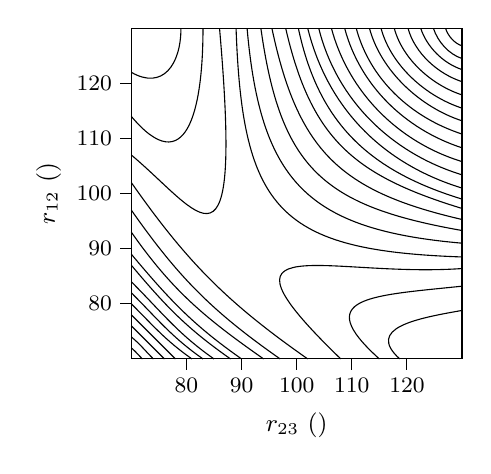
\begin{tikzpicture}[
            % remember picture,overlay,
            % xshift=-4.47cm,yshift=1.08cm,
            % xscale=0.7,yscale=0.73
            scale=0.7
        ]
            \draw (0,0) rectangle (6,6);
    
            \small
            \node at (3,-1.2) {$r_{23}$ (\si{\pico\meter})};
            \node [rotate=90] at (-1.5,3) {$r_{12}$ (\si{\pico\meter})};
    
            \footnotesize
            \draw
                (1,0) -- ++(0,-0.2) node[below]{80}
                (2,0) -- ++(0,-0.2) node[below]{90}
                (3,0) -- ++(0,-0.2) node[below]{100}
                (4,0) -- ++(0,-0.2) node[below]{110}
                (5,0) -- ++(0,-0.2) node[below]{120}
            ;
            \draw
                (0,1) -- ++(-0.2,0) node[left]{80}
                (0,2) -- ++(-0.2,0) node[left]{90}
                (0,3) -- ++(-0.2,0) node[left]{100}
                (0,4) -- ++(-0.2,0) node[left]{110}
                (0,5) -- ++(-0.2,0) node[left]{120}
            ;
    
            \draw
                (0,5.2) to[out=-30,in=-90,looseness=1.4] (0.9,6)
                (0,4.4) to[out=-50,in=-90,looseness=1.9] (1.3,6)
                (0,3.7) to[out=-40,in=-85,out looseness=1.5,in looseness=4.4] (1.6,6)
                %
                (0,3.2) to[out=-55,in=145] (3.2,0)
                (0,2.7) to[out=-55,in=145] (2.7,0)
                (0,2.3) to[out=-55,in=145] (2.4,0)
                (0,1.9) to[out=-50,in=145] (2.0,0)
                (0,1.7) to[out=-50,in=145] (1.8,0)
                (0,1.4) to[out=-45,in=145] (1.5,0)
                (0,1.2) to[out=-45,in=145] (1.3,0)
                (0,1.0) to[out=-45,in=145] (1.1,0)
                (0,0.8) to[out=-45,in=135] (0.8,0)
                (0,0.6) to[out=-45,in=135] (0.6,0)
                (0,0.4) to[out=-40,in=135] (0.4,0)
                (0,0.2) to[out=-40,in=135] (0.2,0)
                %
                (1.90,6) to[out=-88,in=178,looseness=1.45] (6,1.85)
                (2.10,6) to[out=-85,in=175,looseness=1.30] (6,2.1)
                (2.35,6) to[out=-82,in=170,looseness=1.27] (6,2.33)
                (2.55,6) to[out=-78,in=167,looseness=1.19] (6,2.53)
                (2.80,6) to[out=-77,in=163,looseness=1.15] (6,2.73)
                (3.03,6) to[out=-78,in=163,looseness=1.05] (6,2.9)
                (3.20,6) to[out=-76,in=163,looseness=0.95] (6,3.1)
                (3.40,6) to[out=-76,in=163,looseness=0.92] (6,3.34)
                (3.63,6) to[out=-75,in=163,looseness=0.91] (6,3.58)
                (3.87,6) to[out=-75,in=162,looseness=0.91] (6,3.83)
                (4.08,6) to[out=-75,in=162,looseness=0.91] (6,4.08)
                (4.32,6) to[out=-75,in=162,looseness=0.86] (6,4.32)
                (4.53,6) to[out=-75,in=162,looseness=0.86] (6,4.55)
                (4.77,6) to[out=-75,in=162,looseness=0.86] (6,4.79)
                (5.02,6) to[out=-75,in=162,looseness=0.86] (6,5.03)
                (5.25,6) to[out=-72,in=162,looseness=0.86] (6,5.25)
                (5.48,6) to[out=-72,in=162,looseness=0.86] (6,5.45)
                (5.70,6) to[out=-72,in=162,looseness=0.86] (6,5.68)
                %
                (3.80,0) to[out=136,in=-176,out looseness=3.3,in looseness=2.3] (6,1.64)
                (4.50,0) to[out=138,in=-174,looseness=2.15] (6,1.32)
                (4.87,0) to[out=138,in=-170,looseness=1.5] (6,0.88)
            ;
        \end{tikzpicture}
    \end{center}
\end{enumerate}


\subsection*{Application}
\begin{enumerate}[label={\arabic*)}]
    \item Name one HW problem you would like to develop into a thought experiment or relate to a literature article.
    \item Describe how the idea or conclusion from the HW problem applies to the research idea in 1-2 paragraphs (word limit: 300). Once again, this can either be a thought experiment or an experiment found in the literature.
    \item You do not need to derive any equations in this short discussion. Use your intuition and focus on the big picture.
    \item Please cite the literature if you link the HW problem to anyone (author names, titles, journal name, volume numbers, and page numbers).
\end{enumerate}




\end{document}